% Features com rótulo em cada release de teste (Seção Previsão no nível de feature, 03-Metodologia.tex)
% Dados: resultados_e_logs/saida/resultados/nivel_feature_por_release.csv
% Cores usadas nesta figura (valores CMYK da paleta dvipsnames do xcolor), definidas aqui para não depender de opções externas
\definecolor{BurntOrange}{cmyk}{0,0.51,1,0}
\begin{figure}[htbp]
    \centering
    \caption{\textit{Features} com rótulo em cada \textit{release} de teste do protocolo temporal}
    \label{fig:met-features-teste}
    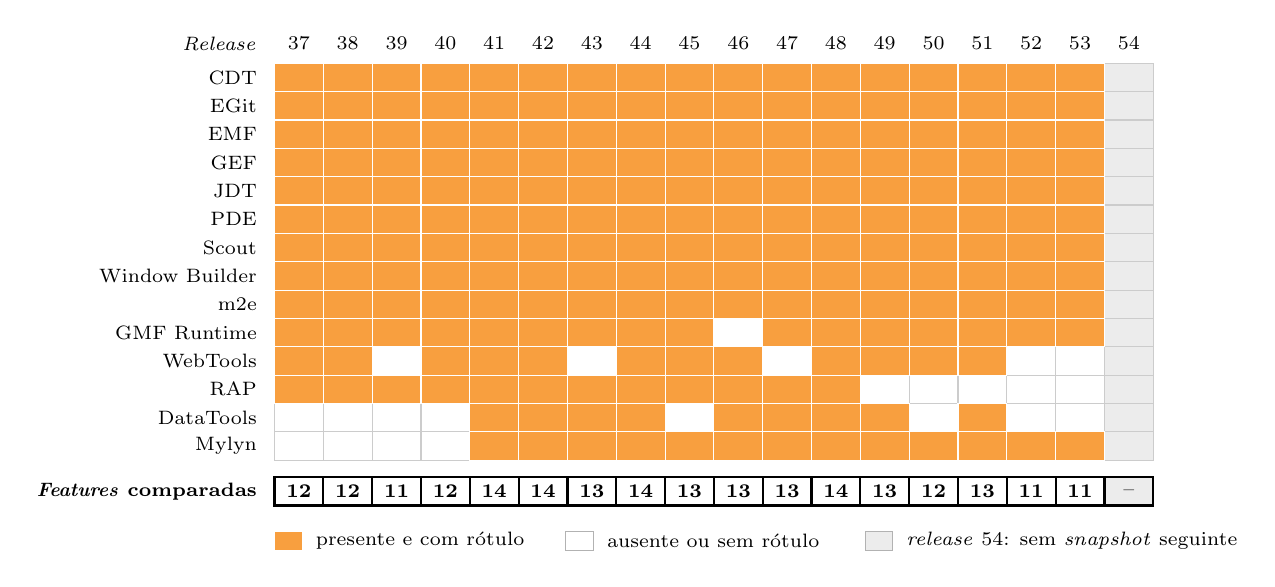
\begin{tikzpicture}[x=1cm,y=1cm,font=\scriptsize]
        \def\w{0.62}
        \def\h{0.36}
        % ---- cabeçalho com as releases
        \node[anchor=east] at (-0.1,0.25) {\textit{Release}};
        \foreach \c in {37,...,54}{\node at ({(\c-37)*\w+\w/2},0.25) {\c};}
        % ---- grade vazia (37 a 53) e coluna 54 sem rótulo
        \foreach \i in {1,...,14}{
            \foreach \c in {37,...,53}{\draw[gray!40] ({(\c-37)*\w},{-\i*\h}) rectangle ++(\w,\h);}
            \filldraw[fill=gray!15,draw=gray!40] ({17*\w},{-\i*\h}) rectangle ++(\w,\h);}
        % ---- células preenchidas: feature presente e com rótulo
        \foreach \nome/\lista [count=\i] in {
                CDT/{37,...,53}, EGit/{37,...,53}, EMF/{37,...,53}, GEF/{37,...,53}, JDT/{37,...,53},
                PDE/{37,...,53}, Scout/{37,...,53}, Window Builder/{37,...,53}, m2e/{37,...,53},
                GMF Runtime/{37,38,39,40,41,42,43,44,45,47,48,49,50,51,52,53},
                WebTools/{37,38,40,41,42,44,45,46,48,49,50,51},
                RAP/{37,...,48},
                DataTools/{41,42,43,44,46,47,48,49,51},
                Mylyn/{41,...,53}}{
            \node[anchor=east] at (-0.1,{-\i*\h+\h/2}) {\nome};
            \foreach \c in \lista{
                \filldraw[fill=BurntOrange!75,draw=white] ({(\c-37)*\w},{-\i*\h}) rectangle ++(\w,\h);}}
        % ---- linha de totais, em forma de vetor
        \node[anchor=east,font=\scriptsize\bfseries] at (-0.1,{-15.6*\h+\h/2}) {\textit{Features} comparadas};
        \foreach \c/\n in {37/12,38/12,39/11,40/12,41/14,42/14,43/13,44/14,45/13,46/13,47/13,48/14,49/13,50/12,
                51/13,52/11,53/11}{
            \draw[thick] ({(\c-37)*\w},{-15.6*\h}) rectangle ++(\w,\h);
            \node[font=\scriptsize\bfseries] at ({(\c-37)*\w+\w/2},{-15.6*\h+\h/2}) {\n};}
        \filldraw[fill=gray!15,thick] ({17*\w},{-15.6*\h}) rectangle ++(\w,\h);
        \node at ({17*\w+\w/2},{-15.6*\h+\h/2}) {--};
        % ---- legenda
        \begin{scope}[shift={(0,{-17.2*\h})}]
            \filldraw[fill=BurntOrange!75,draw=white] (0,0) rectangle ++(0.35,0.25);
            \node[anchor=west] at (0.4,0.125) {presente e com rótulo};
            \draw[gray!60] (3.7,0) rectangle ++(0.35,0.25);
            \node[anchor=west] at (4.1,0.125) {ausente ou sem rótulo};
            \filldraw[fill=gray!15,draw=gray!60] (7.5,0) rectangle ++(0.35,0.25);
            \node[anchor=west] at (7.9,0.125) {\textit{release} 54: sem \textit{snapshot} seguinte};
        \end{scope}
    \end{tikzpicture}
    \fonte{Elaborado pelo autor (2026).}
\end{figure}%
